\documentclass[tikz, border=2mm]{standalone}
\usepackage{tikz}
\usetikzlibrary{calc, arrows.meta}

\definecolor{lineaAzul}{rgb}{0.16, 0.5, 0.72}
\definecolor{lineaRoja}{rgb}{0.9, 0.3, 0.23}

\begin{document}
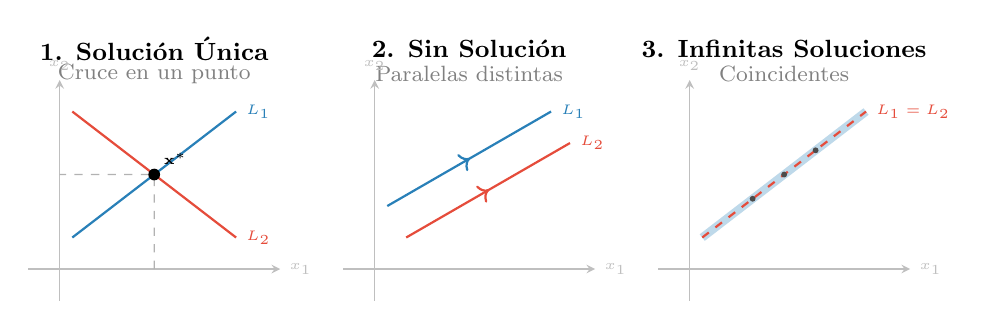
\begin{tikzpicture}[
    scale=0.8,
    axis/.style={->, >=stealth, gray!50, thin},
    linea1/.style={thick, lineaAzul}, 
    linea2/.style={thick, lineaRoja}, 
    dot/.style={circle, fill=black, inner sep=1.5pt}
]

    % --- PANEL 1: SOLUCIÓN ÚNICA ---
    \begin{scope}[shift={(0,0)}]
        \node[font=\bfseries\small] at (1.5, 3.5) {1. Solución Única};
        \node[font=\footnotesize, gray] at (1.5, 3.1) {Cruce en un punto};
        \draw[axis] (-0.5,0) -- (3.5,0) node[right] {\tiny $x_1$};
        \draw[axis] (0,-0.5) -- (0,3) node[above] {\tiny $x_2$};
        \draw[linea1] (0.2, 0.5) -- (2.8, 2.5) node[right] {\tiny $L_1$};
        \draw[linea2] (0.2, 2.5) -- (2.8, 0.5) node[right] {\tiny $L_2$};
        \coordinate (inters) at (1.5, 1.5);
        \draw[dashed, gray!60] (1.5,0) -- (inters) -- (0,1.5);
        \node[dot] at (inters) {};
        \node[above right, font=\tiny] at (inters) {$\mathbf{x}^*$};
    \end{scope}

    % --- PANEL 2: SIN SOLUCIÓN ---
    \begin{scope}[shift={(5,0)}]
        \node[font=\bfseries\small] at (1.5, 3.5) {2. Sin Solución};
        \node[font=\footnotesize, gray] at (1.5, 3.1) {Paralelas distintas};
        \draw[axis] (-0.5,0) -- (3.5,0) node[right] {\tiny $x_1$};
        \draw[axis] (0,-0.5) -- (0,3) node[above] {\tiny $x_2$};
        \draw[linea1] (0.2, 1) -- (2.8, 2.5) node[right] {\tiny $L_1$};
        \draw[linea2] (0.5, 0.5) -- (3.1, 2.0) node[right] {\tiny $L_2$};
        \draw[->, thick, lineaAzul] (1.5, 1.75) -- (1.51, 1.756); 
        \draw[->, thick, lineaRoja] (1.8, 1.25) -- (1.81, 1.256);
    \end{scope}

    % --- PANEL 3: INFINITAS SOLUCIONES ---
    \begin{scope}[shift={(10,0)}]
        \node[font=\bfseries\small] at (1.5, 3.5) {3. Infinitas Soluciones};
        \node[font=\footnotesize, gray] at (1.5, 3.1) {Coincidentes};
        \draw[axis] (-0.5,0) -- (3.5,0) node[right] {\tiny $x_1$};
        \draw[axis] (0,-0.5) -- (0,3) node[above] {\tiny $x_2$};
        \draw[linea1, line width=3pt, opacity=0.3] (0.2, 0.5) -- (2.8, 2.5);
        \draw[linea2, dashed, thick] (0.2, 0.5) -- (2.8, 2.5) node[right] {\tiny $L_1 = L_2$};
        \foreach \x in {1, 1.5, 2} {
            \node[dot, scale=0.5, fill=black!70] at (\x, {(\x-0.2)/2.6*2 + 0.5}) {};
        }
    \end{scope}

\end{tikzpicture}
\end{document}
